
We provide here additional information on the combination inputs and results.
Figure~\ref{fig:pdfcorr2} shows the correlation matrices for the hadron-collider measurements 
for the CT14, MMHT2014, NNPDF3.1 PDF sets.  Tables~\ref{tbl:wgttev}--\ref{tbl:wgtall} give
the relative weight of each measurement to various combinations of measurements.

\begin{figure}[!tbp]
   \centering
        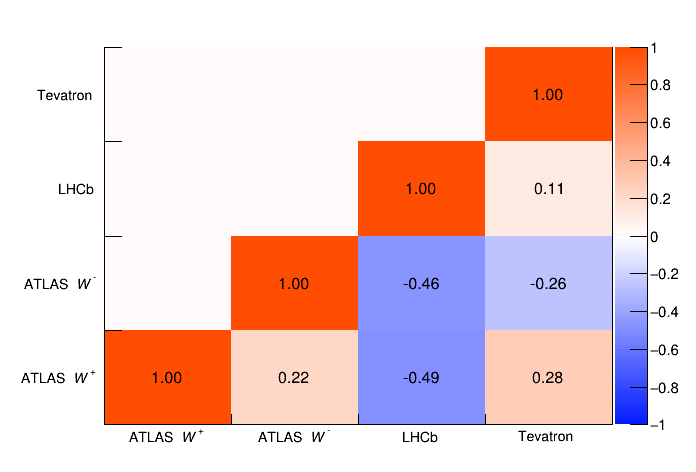
\includegraphics[width=0.9\columnwidth]{13000_CT14nnlo_ATLAS_LHCb_CDF9fb_D05fb_LEP_combination.root_rebin.png}
        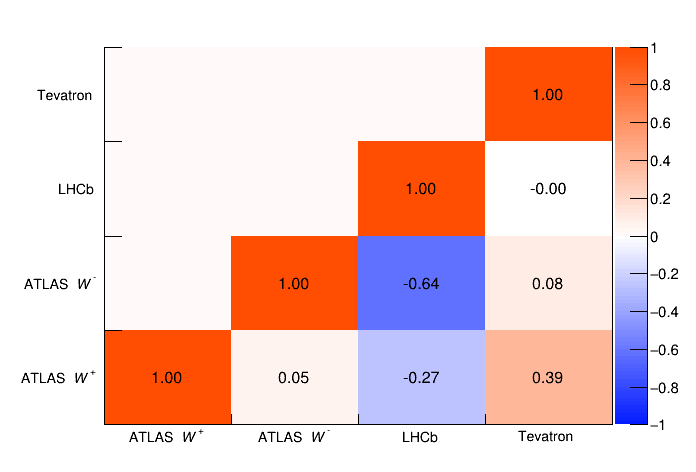
\includegraphics[width=0.9\columnwidth]{25300_MMHT2014nnlo68cl_ATLAS_LHCb_CDF9fb_D05fb_LEP_combination.root_rebin.png}
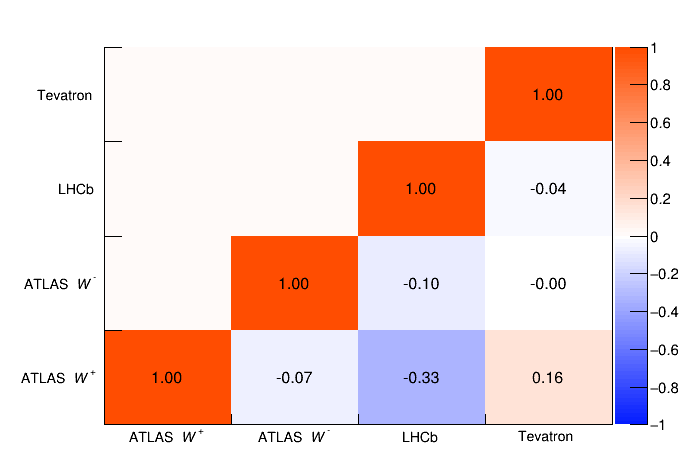
\includegraphics[width=0.9\columnwidth]{304400_NNPDF31_nnlo_as_0118_hessian_ATLAS_LHCb_CDF9fb_D05fb_LEP_combination.root_rebin.png}
\caption{PDF uncertainty correlation matrices for the CT14, MMHT2014, and NNPDF3.1 PDF sets, shown from top to bottom.
}
\label{fig:pdfcorr2}
\end{figure}

\begin{table*}[!tbp]
  \centering
  \begin{tabular}{l@{\extracolsep{\fill}}rrrrrrrr}
  \hline \hline
          Measurement         & &   ABMP16  &  CT14  &    CT18  &  MMHT2014  &  MSHT20  &   NNPDF3.1  &   NNPDF4.0 \\
\hline 
                      CDF     & &   85.3  &    86.8  &    88.1  &    86.4  &    86.3  &    86.2  &    86.1 \\
                      D0      & &   14.7  &    13.2  &    11.9  &    13.6  &    13.7  &    13.8  &    13.9 \\
\hline \hline 
\end{tabular}

  \caption{Relative weights (in percent) of the CDF and D0 measurements for the Tevatron combination.}
\label{tbl:wgttev}
\end{table*}

\begin{table*}[!tbp]
  \centering
  \begin{tabular}{l@{\extracolsep{\fill}}rrrrrrrr}
  \hline \hline
Measurement       &  &  ABMP16  &    CT14  &      CT18  &  MMHT2014  &    MSHT20  &   NNPDF3.1  &   NNPDF4.0 \\
\hline 
         ATLAS    &  &    77.8  &    69.3  &    70.5  &    72.4  &    73.7  &    74.9  &    77.0 \\
         LHCb     &  &    22.2  &    30.7  &    29.5  &    27.6  &    26.3  &    25.1  &    23.0 \\
\hline \hline
\end{tabular}

  \caption{Relative weights (in percent) of the ATLAS and LHCb measurements for the LHC combination.}
\label{tbl:wgtlhc}
\end{table*}

\begin{table*}[!tbp]
  \centering
  \begin{tabular}{l@{\extracolsep{\fill}}rrrrrrrr}
  \hline \hline
Measurement                 &     &    ABMP16  &      CT14  &      CT18  &  MMHT2014  &    MSHT20  &   NNPDF3.1  &   NNPDF4.0 \\
\hline
                      ATLAS &     &    19.9  &    28.2  &    28.2  &    20.2  &    22.8  &    19.7  &    24.8 \\
                      LHCb  &     &     6.0  &    12.7  &    13.4  &     9.7  &    10.7  &     8.5  &     8.9 \\
                      CDF   &  &    58.8  &    42.2  &    41.1  &    54.0  &    50.6  &    56.1  &    51.0 \\
                      D0    &  &    10.1  &     6.0  &     5.1  &     8.3  &     7.9  &     8.7  &     8.1 \\
                      LEP   &     &     5.2  &    10.9  &    12.2  &     7.7  &     8.0  &     7.0  &     7.2 \\
\hline \hline
\end{tabular}

  \caption{Relative weights (in percent) of individual measurements 
    for the combination of all available measurements.}
\label{tbl:wgtall}
\end{table*}

\begin{table*}[!tbp]
  \centering
  \begin{tabular}{l@{\extracolsep{\fill}}rrrrrrrr}
  \hline \hline
Measurement                     &  &  ABMP16  &      CT14  &      CT18  &  MMHT2014  &    MSHT20  &   NNPDF3.1  &   NNPDF4.0 \\
\hline 
                          ATLAS  &    &    21.0  &    31.6  &    32.1  &    21.9  &    24.7  &    21.2  &    26.7 \\
                          LHCb   &    &     6.3  &    14.3  &    15.3  &    10.5  &    11.7  &     9.1  &     9.5 \\
                          CDF    & &    62.1  &    47.3  &    46.8  &    58.6  &    55.0  &    60.4  &    55.0 \\
                          D0     & &    10.6  &     6.7  &     5.8  &     9.0  &     8.6  &     9.3  &     8.7 \\
\hline \hline 
\end{tabular}

  \caption{Relative weights (in percent) of individual measurements 
    for the combination of all except the LEP measurement.}
\label{tbl:wgtallexclep}
\end{table*}

\begin{table*}[!tbp]
  \centering
  \begin{tabular}{l@{\extracolsep{\fill}}rrrrrrrr}
  \hline \hline
Measurement             &               &    ABMP16  &      CT14  &      CT18  &  MMHT2014  &    MSHT20  &   NNPDF3.1  &   NNPDF4.0 \\
\hline 
                           ATLAS   &   &    47.4  &    41.5  &    42.2  &    42.5  &    44.2  &    44.4  &    47.5 \\
                          LHCb  &     &    13.7  &    18.6  &    18.4  &    17.1  &    17.0  &    15.8  &    14.9 \\
                          D0 &    &    27.5  &    24.6  &    23.1  &    26.9  &    25.7  &    26.8  &    25.3 \\
                        LEP  &      &    11.5  &    15.3  &    16.2  &    13.5  &    13.1  &    13.0  &    12.4 \\
\hline \hline 
\end{tabular}

  \caption{Relative weights (in percent) of individual measurements 
    for the combination of all except the CDF measurement.}
\label{tbl:wgtallexccdf}
\end{table*}

\begin{table*}[!tbp]
  \centering
  \begin{tabular}{l@{\extracolsep{\fill}}rrrrrrrr}
  \hline \hline
Measurement        &                &    ABMP16  &      CT14  &      CT18  &  MMHT2014  &    MSHT20  &   NNPDF31  &   NNPDF40 \\
\hline
                           ATLAS &     &    21.9  &    28.8  &    28.7  &    21.5  &    24.0  &    21.3  &    26.2 \\
                              LHCb  &     &     6.5  &    13.0  &    13.6  &    10.1  &    11.1  &     8.9  &     9.2 \\
                         CDF  &  &    66.0  &    47.2  &    45.4  &    60.4  &    56.7  &    62.5  &    57.1 \\
                               LEP    &    &     5.6  &    11.1  &    12.3  &     8.0  &     8.2  &     7.3  &     7.5 \\
\hline \hline 
\end{tabular}

  \caption{Relative weights (in percent) of individual measurements 
    for the combination of all except the D0 measurement.}
\label{tbl:wgtallexcd0}
\end{table*}

\begin{table*}[!tbp]
  \centering
  \begin{tabular}{l@{\extracolsep{\fill}}rrrrrrrr}
  \hline \hline
Measurement &               &    ABMP16  &      CT14  &      CT18  &  MMHT2014  &    MSHT20  &   NNPDF3.1  &   NNPDF4.0 \\
\hline
LHCb   &    &     7.2  &    14.8  &    15.7  &    10.4  &    12.1  &     9.4  &    11.0 \\
                CDF   &  &    73.8  &    61.0  &    60.4  &    69.5  &    67.4  &    71.0  &    68.7 \\
                         D0    &  &    12.7  &     9.2  &     7.9  &    10.9  &    10.7  &    11.3  &    11.1 \\
                                 LEP &       &     6.3  &    15.0  &    16.0  &     9.2  &     9.8  &     8.3  &     9.2 \\
\hline \hline 
\end{tabular}

  \caption{Relative weights (in percent) of individual measurements 
    for the combination of all except the ATLAS measurement.}
\label{tbl:wgtallexcatlas}
\end{table*}

\begin{table*}[!tbp]
  \centering
  \begin{tabular}{l@{\extracolsep{\fill}}rrrrrrrr}
  \hline \hline
Measurement  &   &    ABMP16  &      CT14  &      CT18  &  MMHT2014  &    MSHT20  &   NNPDF3.1  &   NNPDF4.0 \\
\hline 
                   ATLAS  &    &    21.0  &    30.1  &    30.7  &    21.1  &    24.6  &    21.0  &    27.1 \\
                   CDF &      &    62.7  &    50.0  &    48.8  &    60.8  &    57.3  &    61.7  &    56.1 \\
                   D0   &   &    10.8  &     7.2  &     6.2  &     9.4  &     9.0  &     9.6  &     8.9 \\
                 LEP  &      &     5.5  &    12.7  &    14.2  &     8.7  &     9.1  &     7.7  &     8.0 \\
\hline \hline
\end{tabular}

  \caption{Relative weights (in percent) of individual measurements 
    for the combination of all except the LHCb measurement.}
\label{tbl:wgtallexclhcb}
\end{table*}
